\documentclass[a4paper]{article}
\linespread{1.6}
\usepackage{geometry}
\usepackage{setspace}
\usepackage{amsmath}
\usepackage{amssymb}
\usepackage{enumerate}
\usepackage[pdftex]{graphicx}
\usepackage{float}
\usepackage{subfigure}
\usepackage{listings}
\geometry{left=1.5cm,right=1.5cm,top=2.5cm,bottom=2.5cm}

\begin{document}
\begin{spacing}{2.0}
\begin{flushleft}\begin{huge}EEE5502 Foundations of Digital Signal Processing   Code 6\end{huge}\end{flushleft}
\begin{flushright}\begin{Large} Hudanyun Sheng \end{Large}\end{flushright}

\Large\textbf{ Question \#1}:  \\
\normalsize
I spent 10 hours.\\

\Large\textbf{Question \#2}:  
\normalsize
\begin{enumerate}[(a)]
\item System 1 would cutoff the input signals if the magnitude of the input signal is smaller than 20(outputs 0), would output the original when the magnitude is greater than 20. 

\item System 2 is a low pass filter.

\item The behavior of system 2 is shown in the approximate DTFT in the plot below, and it proves that system 2 is a low pass filter.
\begin{figure} [H]
\centering
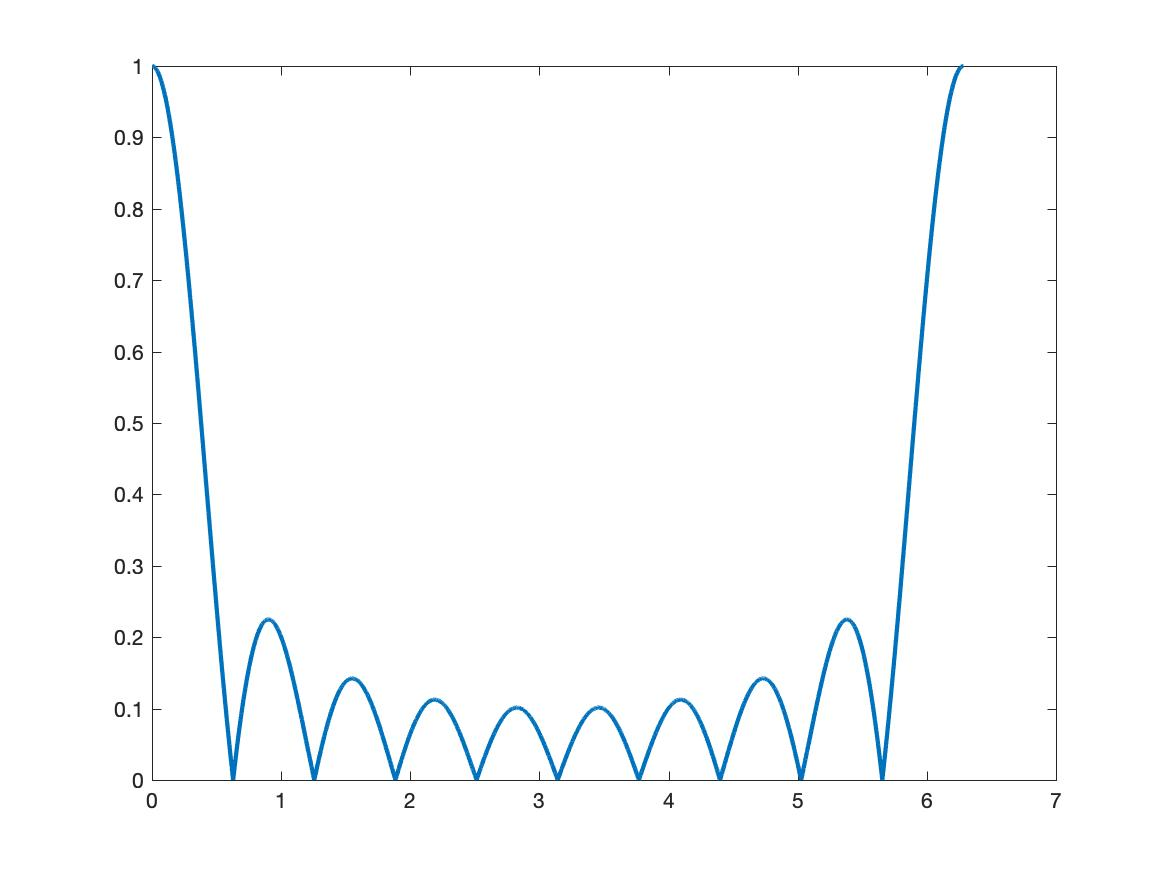
\includegraphics[width=3in]{2c.jpg}
\label{fig:graph}
\end{figure}

\item The ploe-zero plot of system 3 is shown below:
\begin{figure} [H]
\centering
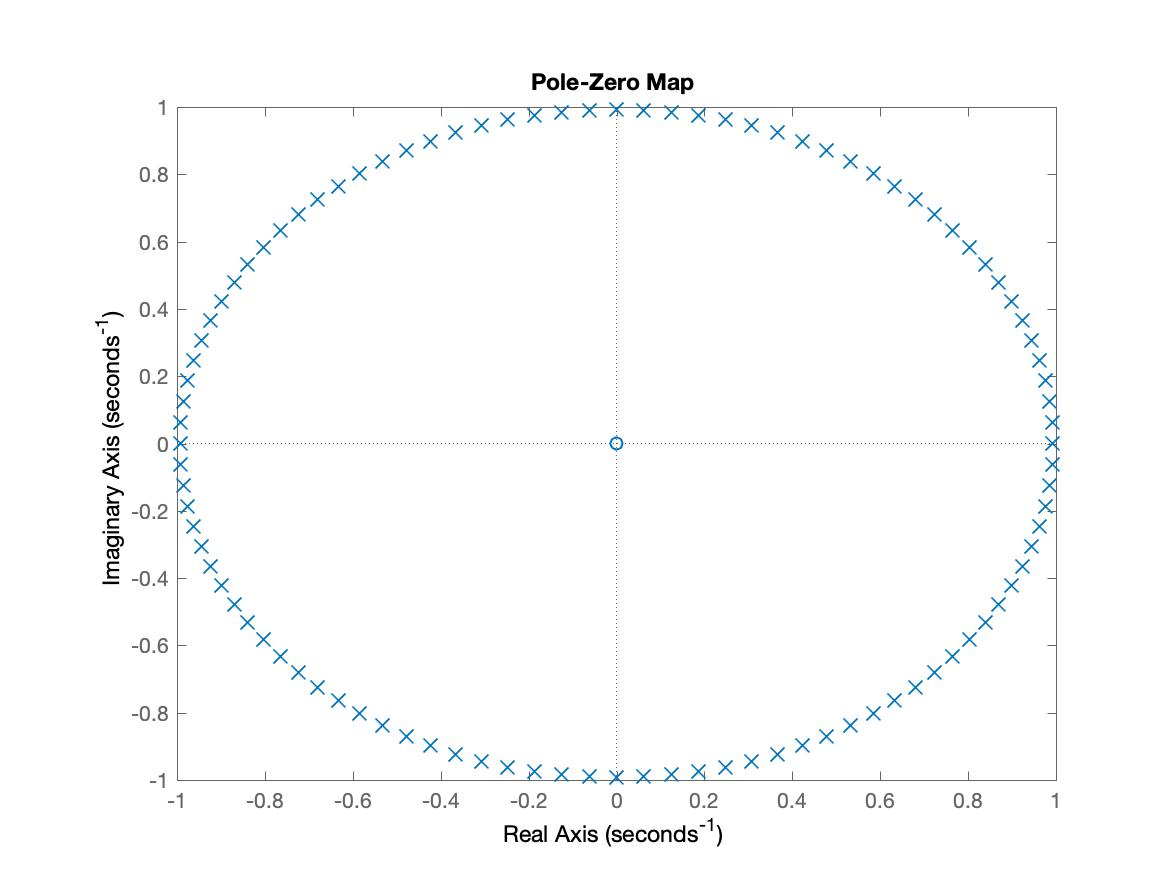
\includegraphics[width=3in]{2d.jpg}
\label{fig:graph}
\end{figure}

\item System 3 is an all pass filter.

\item System 3 would pass all the input signal.
\end{enumerate}


\Large\textbf{Question \#3}:  
\normalsize
\begin{enumerate}[(a)]
\item The STFT of the original signal ``chiptune\_noise" after system 1 applied across the frequency domain is shown below:
\begin{figure}[H]
\centering
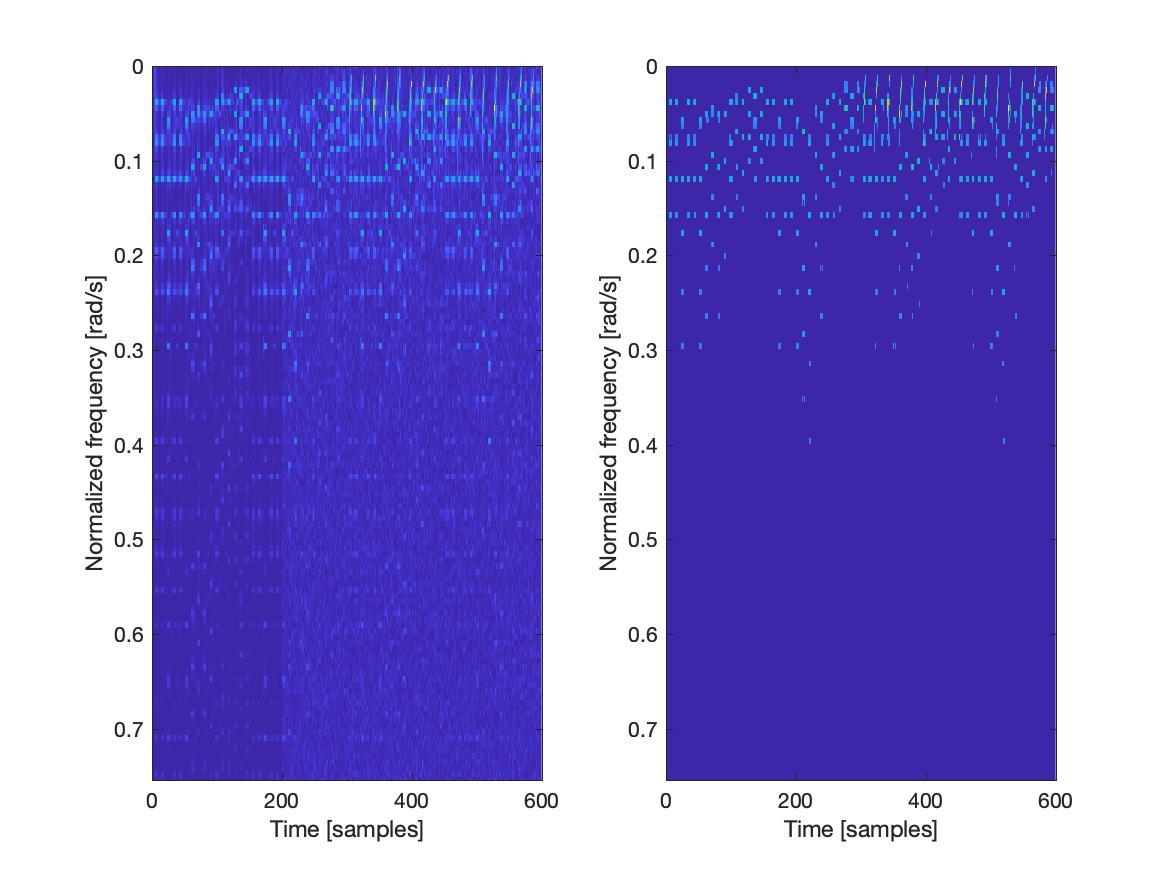
\includegraphics[width=5in]{3a.jpg}
\label{fig:graph}
\end{figure}
The original audio signal and the modified signal is shown below in the same figure:
\begin{figure}[H]
\centering
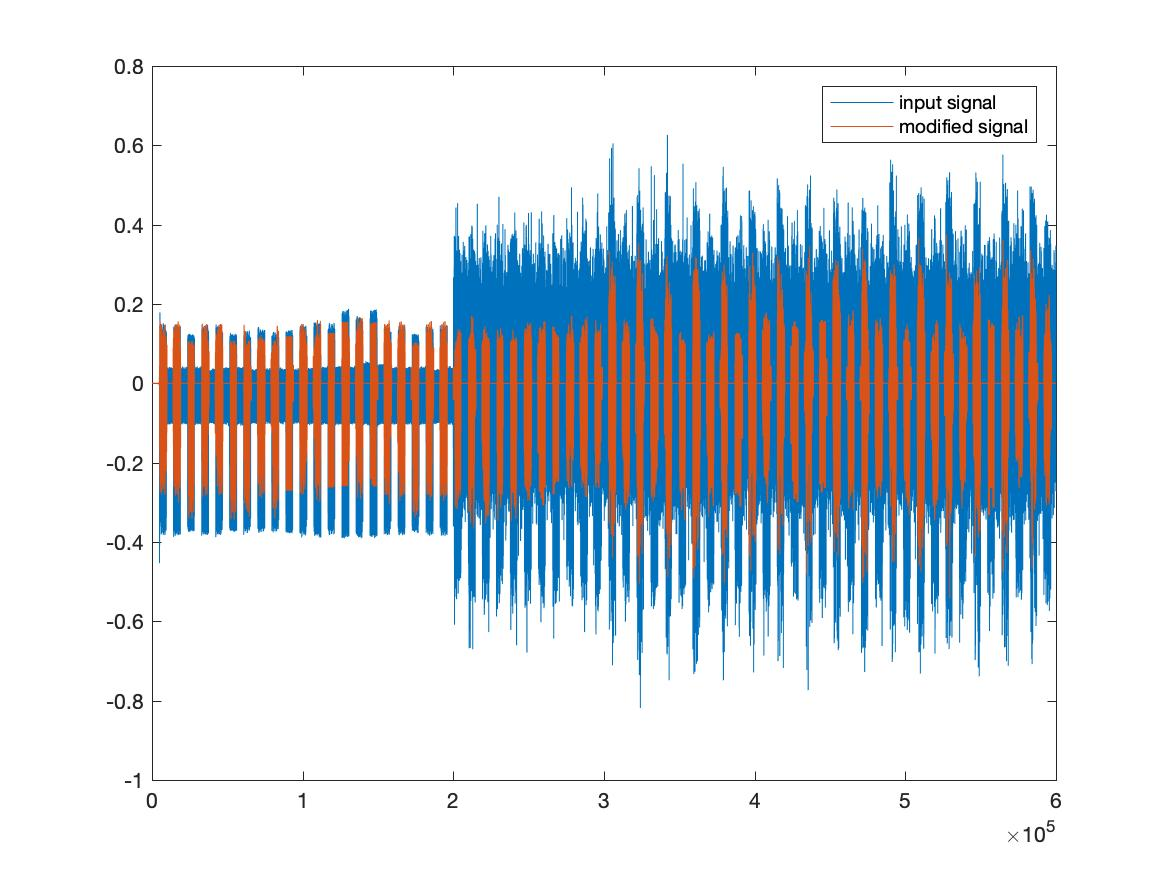
\includegraphics[width=5in]{3a_audio.jpg}
\label{fig:graph}
\end{figure}

\item The STFT of the original signal ``chiptune\_normal" after system 2 applied over the time domain of the STFT is shown below:
\begin{figure}[H]
\centering
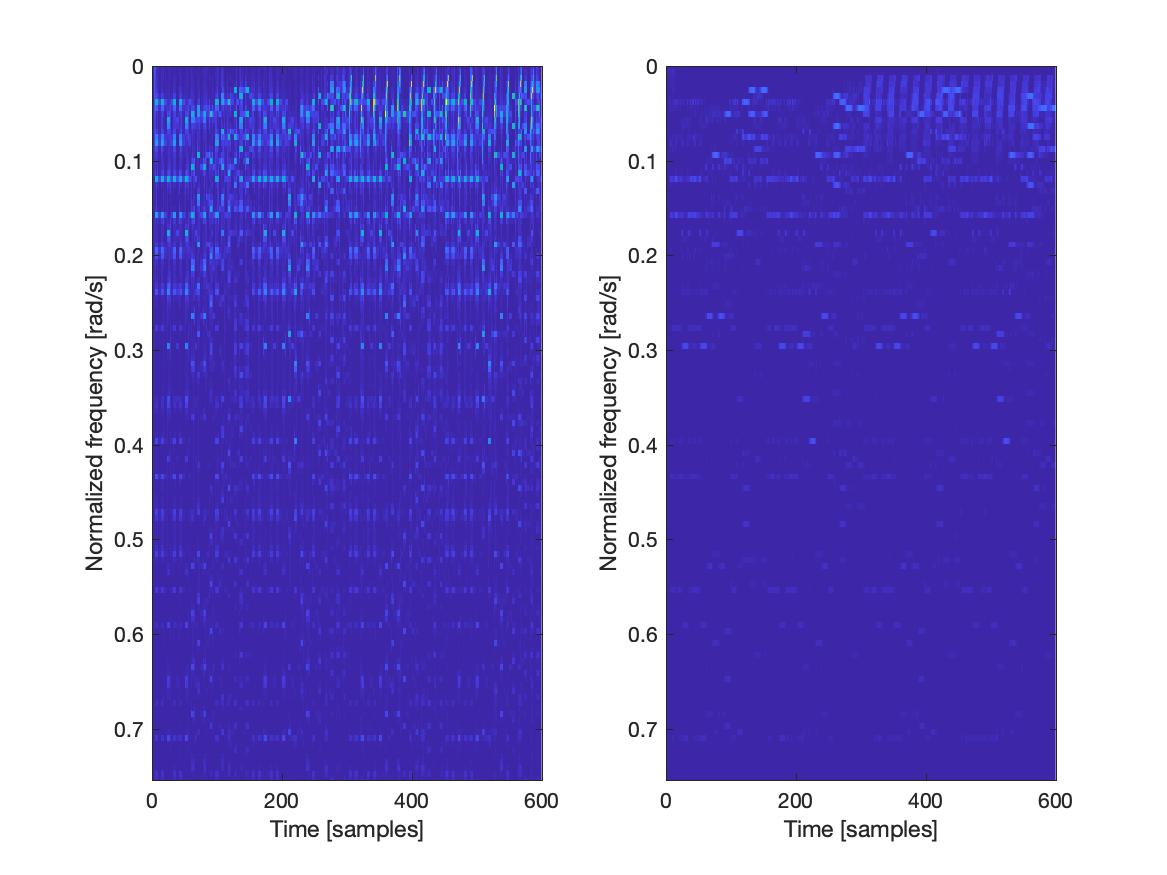
\includegraphics[width=5in]{3b.jpg}
\label{fig:graph}
\end{figure}
The original audio signal and the modified signal is shown below in the same figure:
\begin{figure}[H]
\centering
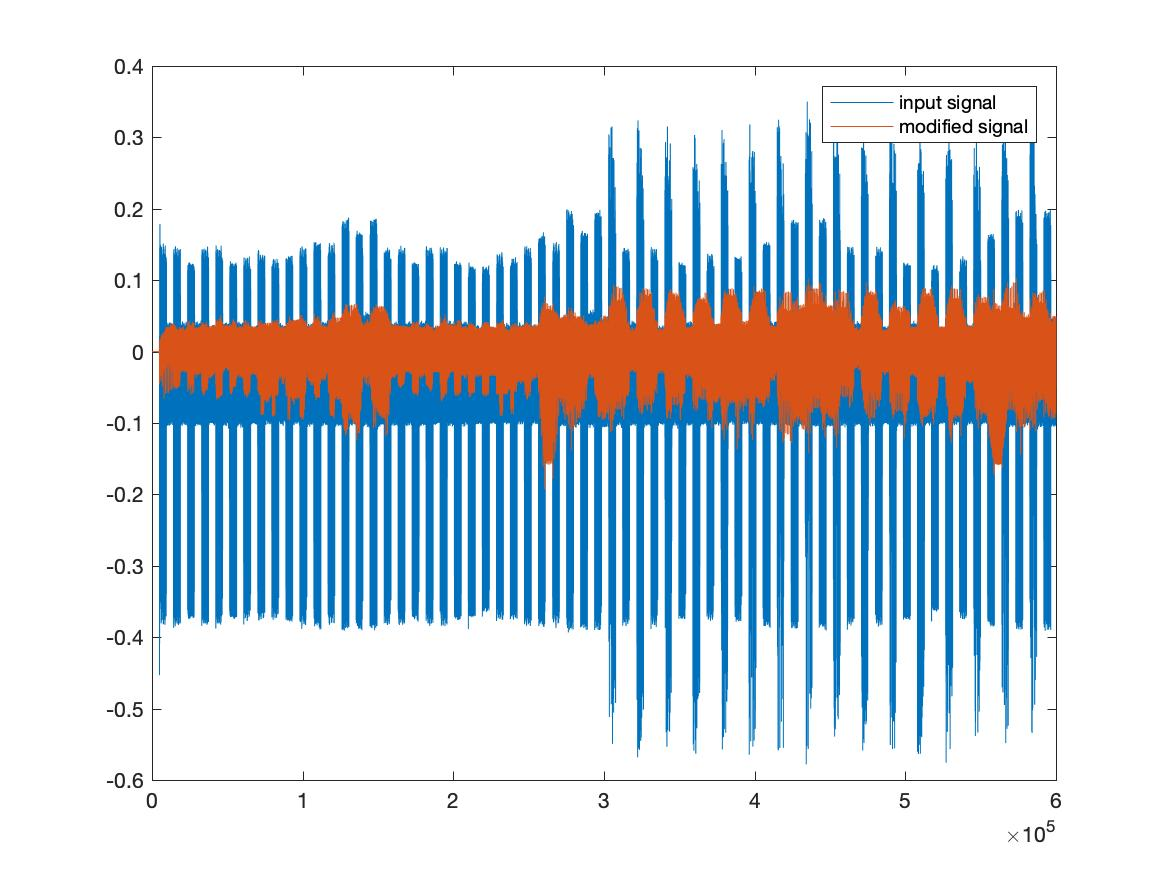
\includegraphics[width=5in]{3b_audio.jpg}
\label{fig:graph}
\end{figure}

\item The STFT of the original signal ``chiptune\_noaudio" after system 3 applied over the time domain os the STFT is shown below:
\begin{figure}[H]
\centering
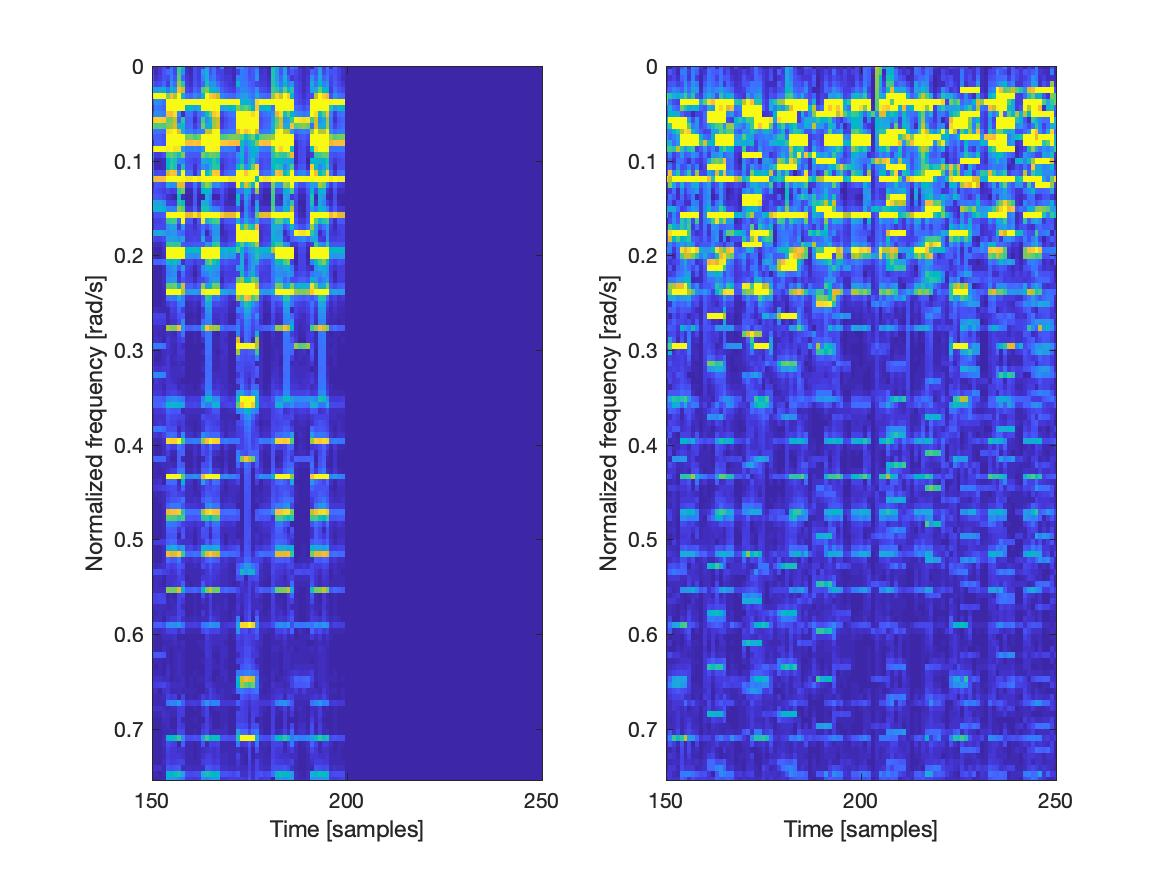
\includegraphics[width=5in]{3c.jpg}
\label{fig:graph}
\end{figure}
The original audio signal and the modified signal is shown below in the same figure:
\begin{figure}[H]
\centering
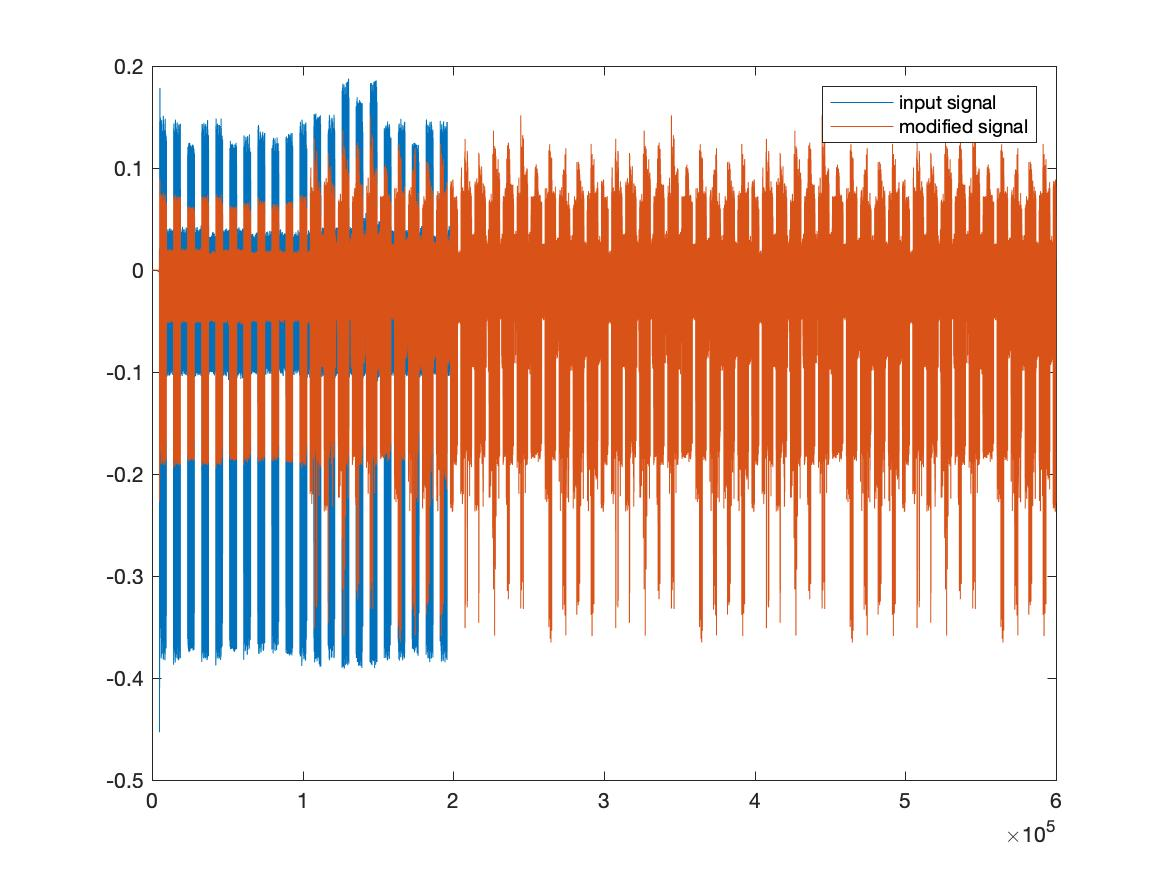
\includegraphics[width=5in]{3c_audio.jpg}
\label{fig:graph}
\end{figure}


\end{enumerate}

\Large\textbf{Question \#4}:  
\normalsize
\begin{enumerate}[(a)]
\item The STFT of the original signal ``chiptune\_noise" after system 1 applied across the frequency domain and with the overlap-add STFT is shown below:
\begin{figure}[H]
\centering
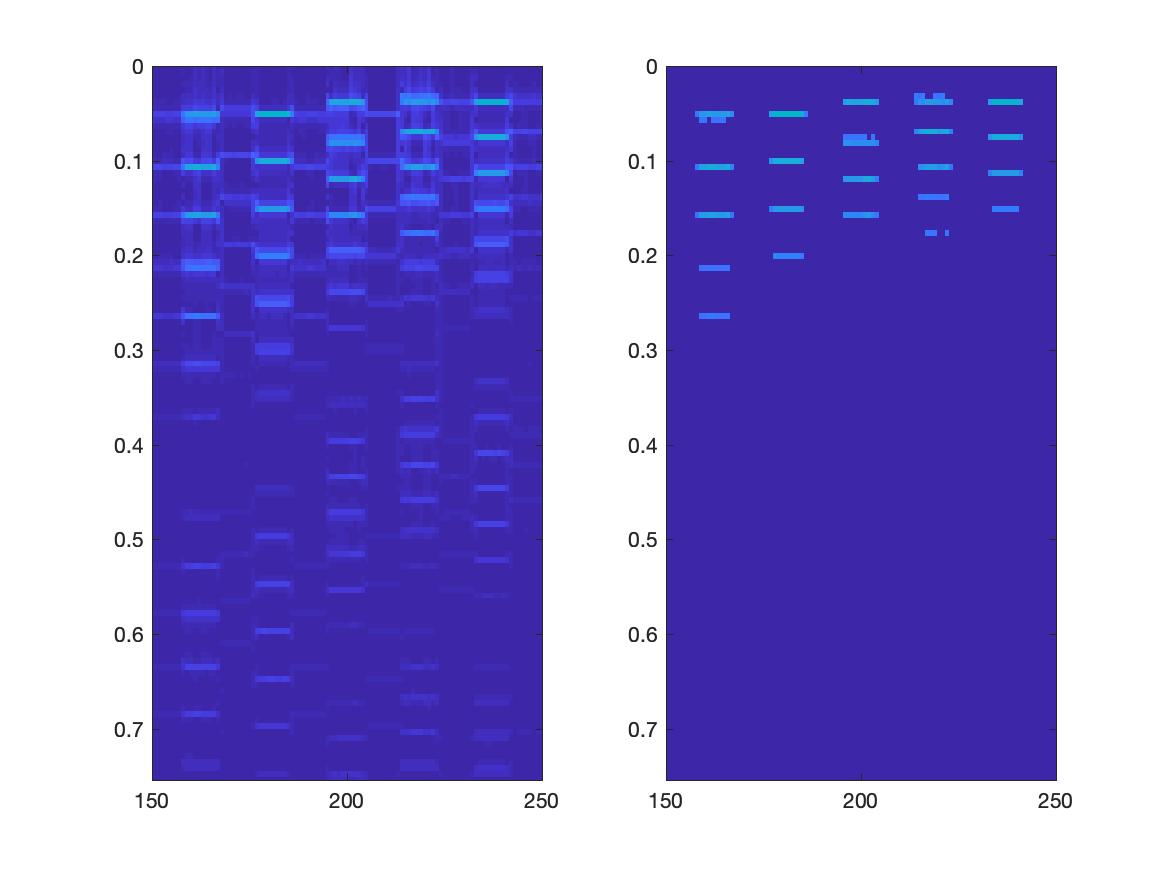
\includegraphics[width=5in]{4a.jpg}
\label{fig:graph}
\end{figure}
The original audio signal and the modified signal is shown below in the same figure:
\begin{figure}[H]
\centering
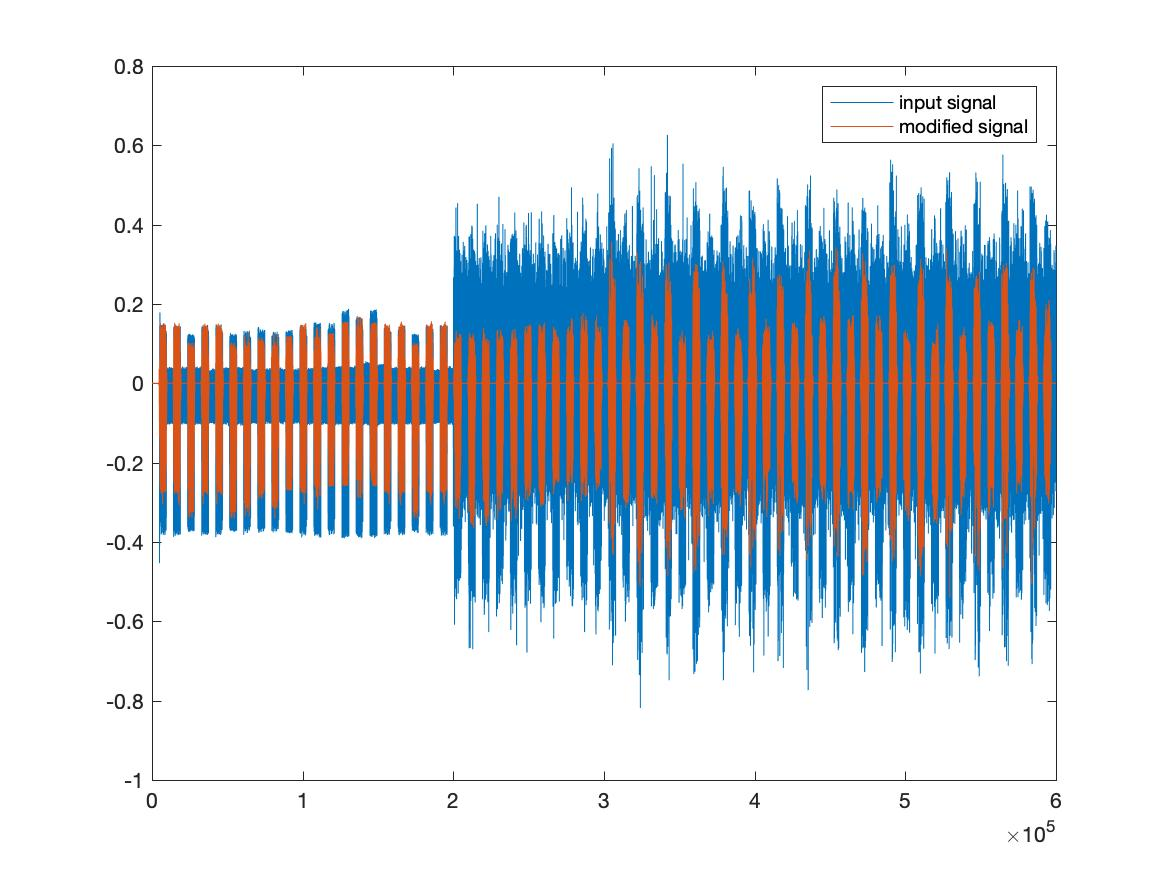
\includegraphics[width=5in]{4a_audio.jpg}
\label{fig:graph}
\end{figure}

\item The STFT of the original signal ``chiptune\_normal" after system 2 applied across the frequency domain and with the overlap-add STFT is shown below:
\begin{figure}[H]
\centering
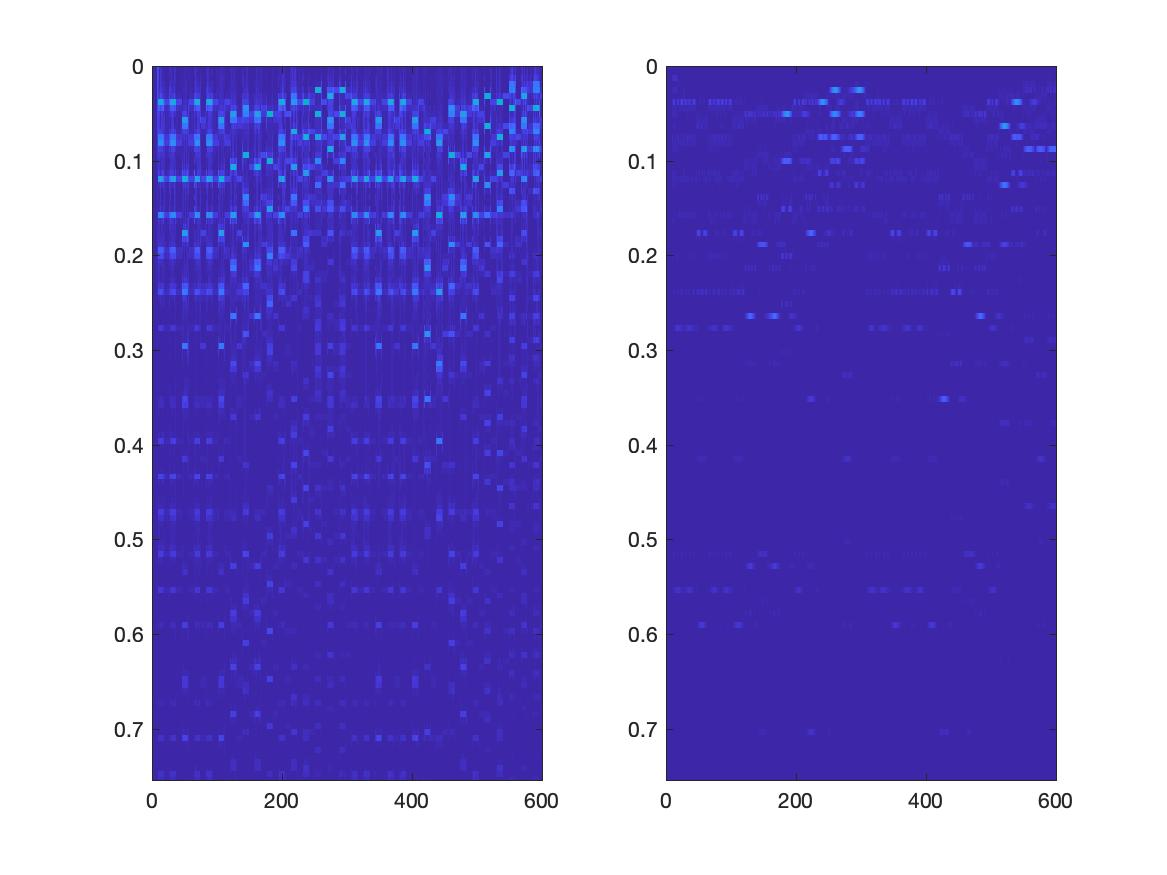
\includegraphics[width=5in]{4b.jpg}
\label{fig:graph}
\end{figure}
The original audio signal and the modified signal is shown below in the same figure:
\begin{figure}[H]
\centering
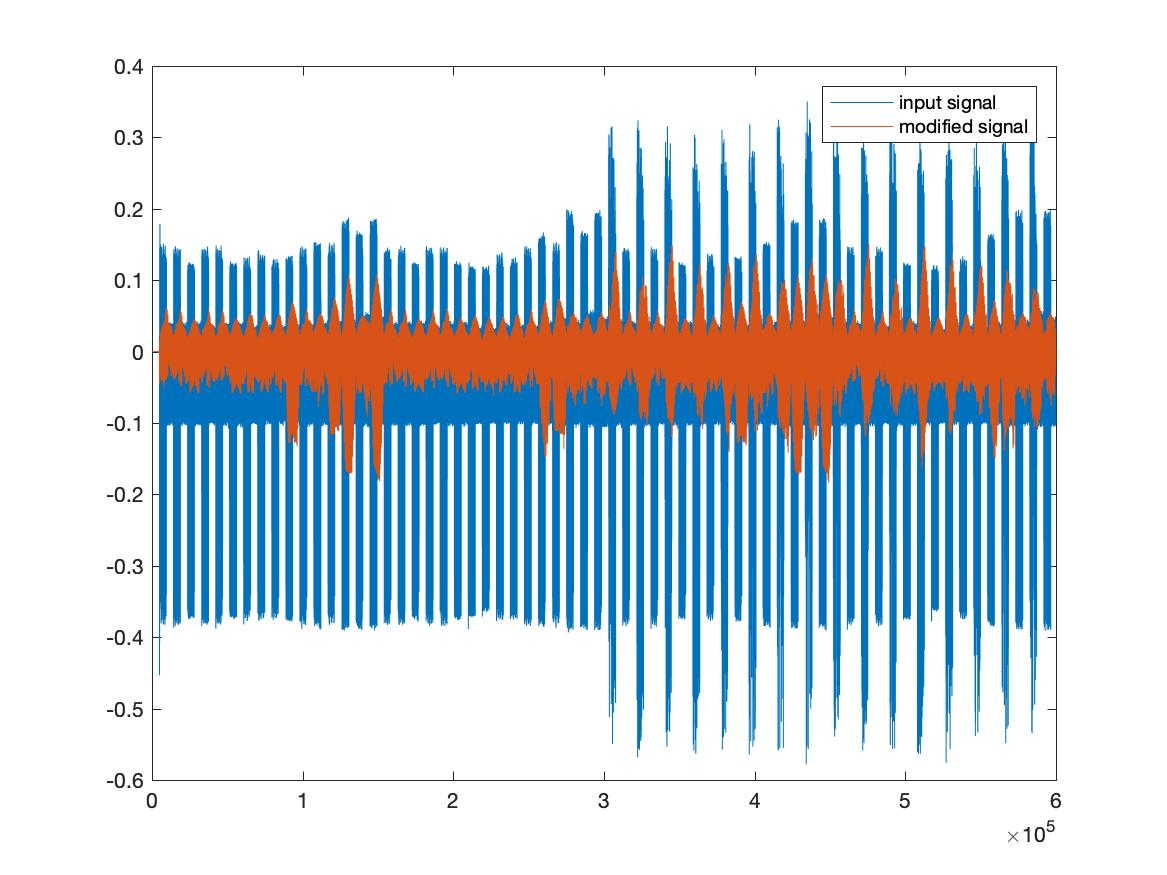
\includegraphics[width=5in]{4b_audio.jpg}
\label{fig:graph}
\end{figure}

\item The STFT of the original signal ``chiptune\_normal" after system 3 applied across the frequency domain and with the overlap-add STFT is shown below:
\begin{figure}[H]
\centering
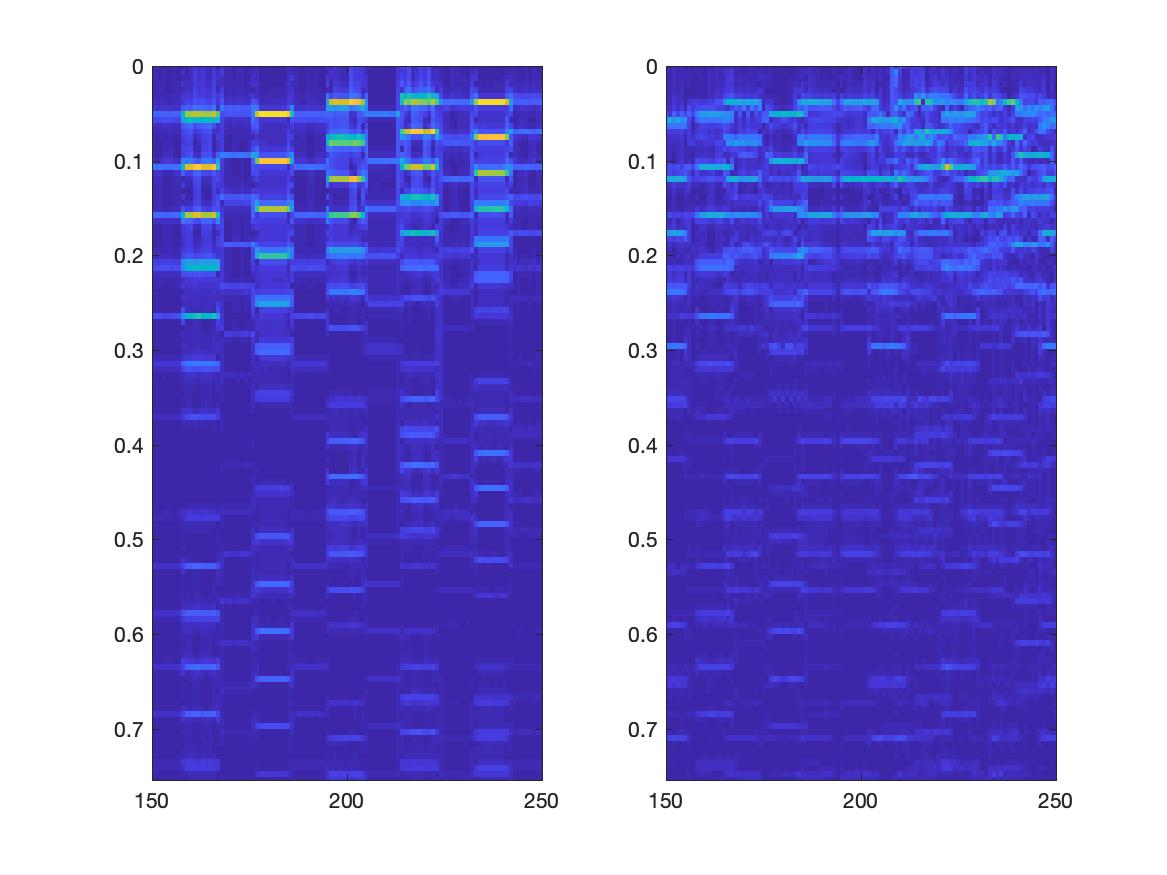
\includegraphics[width=5in]{4c.jpg}
\label{fig:graph}
\end{figure}
The original audio signal and the modified signal is shown below in the same figure:
\begin{figure}[H]
\centering
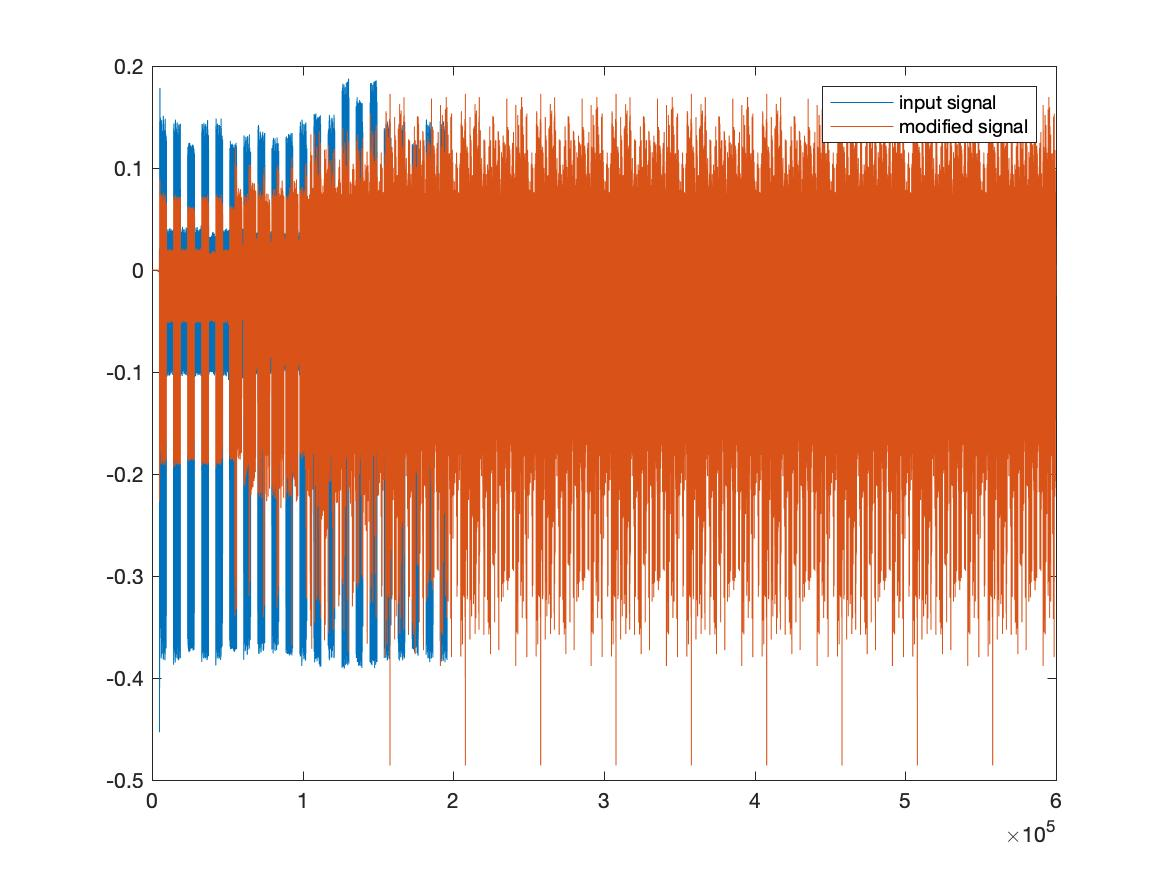
\includegraphics[width=5in]{4c_audio.jpg}
\label{fig:graph}
\end{figure}
\end{enumerate}



\end{spacing}
\end{document}